\textbf{Ensembles.} Ensemble learning is then performed on the labels by generated 8 classifers, including $k$-NN with euclidean, $k$-NN with chi-square, SVM-linear (-t 0), SVM-$\chi^2$ (-t 5), SVM-RBF (-c 4000 -g 15 -t 2), linear SVM (-c 40), polynomial SVM (-c 1000 -g 1 -d 2 -t 1), sigmoid SVM (-c 1000 -g 1 -d 2 -t 3). We take 4/5 examples as training samples, and 1/5 examples as testing examples.


Figure \ref{fig:diversity_k} gives the training and testing accuracy for the nine measures of diversity (1. \emph{disagreement}, 2. \emph{correlation coefficient}, 3. \emph{Q-statistic}, 4. \emph{double-fault}, 5. \emph{coincident failure diversity}, 6. \emph{entropy}, 7. \emph{interrater agreement}, 8. \emph{Kohavi-Wolpert}, and 9. \emph{generalized diversity}) in different $\tilde{K}$ values, where $C\text{-strategy}$ is uniform, and $B\text{-strategy}$ is the basic form. Accuracy increases as $\tilde{K}$ increases, which might due to $K$ is not sufficently large. However, the test accuracy can be better as
$\tilde{K}=5$ for some measures of diversity.

\begin{figure} [t]
\centering
\begin{subfigure}{.40\textwidth}
  \centering
  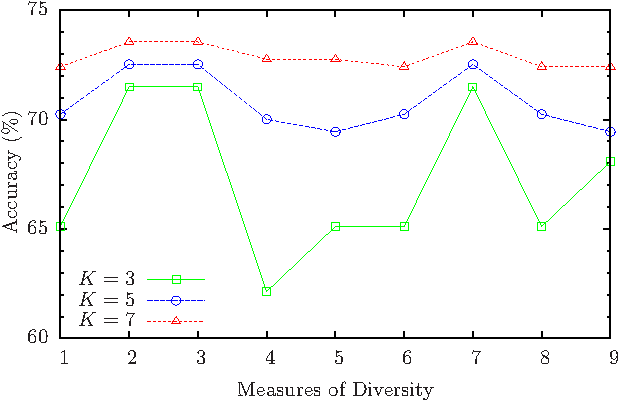
\includegraphics[width=.90\linewidth]{../Figure/diversity_k_train}
  \caption{Training Accuracy}
  \label{fig:diversity_k_train}
\end{subfigure}%
\begin{subfigure}{.40\textwidth}
  \centering
  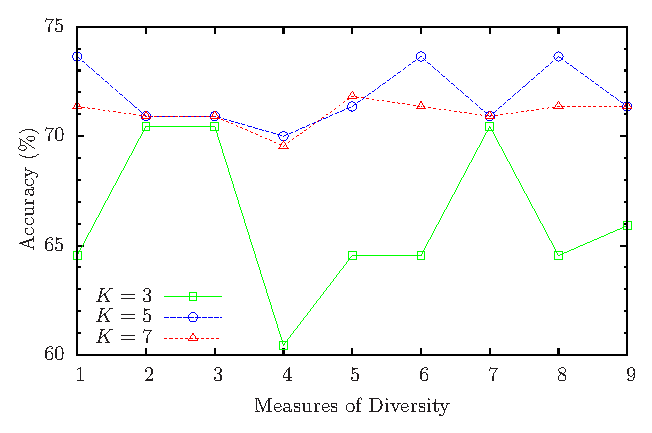
\includegraphics[width=.90\linewidth]{../Figure/diversity_k_test}
  \caption{Testing Accuracy}
  \label{fig:diversity_k_test}
\end{subfigure}
\caption{Training and testing accuracy for different measures of diversity in different $\tilde{K}$ values.}
\label{fig:diversity_k}
\end{figure}

Figure \ref{fig:diversity_0.7_others} gives the training and testing accuracy for different measures of diversity in different $C\text{-strategy}$ and $B\text{-strategy}$, where $\tilde{K}=7$. The new form of $B\text{-strategy}$ can lead to better testing accuracy for some measures of diversity, although does not help on training accuracy.

%Accuracy increases as $\tilde{K}$ increases, which might due to $K$ is not sufficently large. However, the test accuracy can be better as
%$\tilde{K}=5$ for some measures of diversity.

\begin{figure} [t]
\centering
\begin{subfigure}{.40\textwidth}
  \centering
  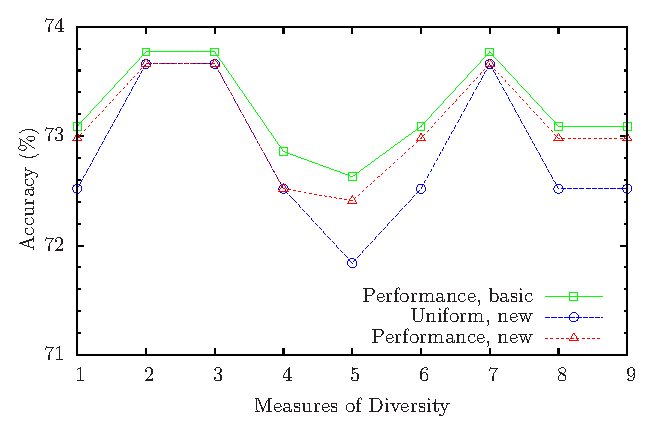
\includegraphics[width=.90\linewidth]{../Figure/diversity_7_others_train}
  \caption{Training Accuracy}
  \label{fig:diversity_0.7_others_train}
\end{subfigure}%
\begin{subfigure}{.40\textwidth}
  \centering
  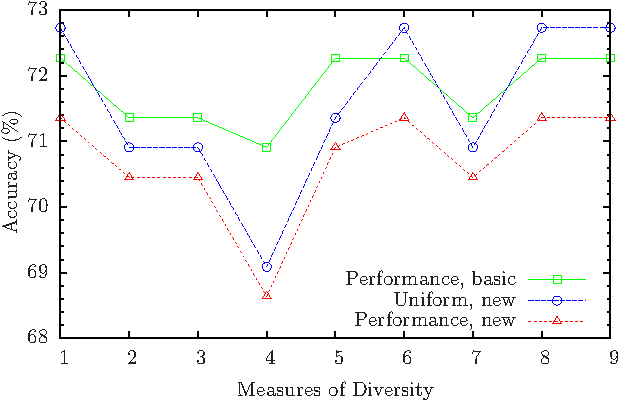
\includegraphics[width=.90\linewidth]{../Figure/diversity_7_others_test}
  \caption{Testing Accuracy}
  \label{fig:diversity_0.7_others_test}
\end{subfigure}
\caption{Training and testing accuracy for different measures of diversity in different $\tilde{K}$ values.}
\label{fig:diversity_0.7_others}
\end{figure}


The optimization method using DEPSO is performed as $\tilde{K}=|K|$. For the basic and new forms of $B\text{-strategy}$, it respectively obtained 75.26\% and 71.82\% training and testing accuracy, and 75.26\% and 71.36\% training and testing accuracy. This gives the best training accuracy is 75.26\%, and it does not lead to higher test accuracy.

Figure \ref{fig:threshoulds} gives the classification accuracy and rates for different $C\text{-strategy}$ methods in different $\bar{V}$ values, where $\tilde{K}=|K|$, with the \emph{new form} of $B\text{-strategy}$, on testing examples. In general, the accuracy accuracy increases and classification rate decreases, as $\bar{V}$ increases. However, there is a drop at $\bar{V}=0.8$, which means the base classifers may reach agreements on some wrong labels. The optimizion method can keep the classification rate higher, especially in the high accuracy region. For example, for $\bar{V}=0.7$, there is a nearly 95\% accuracy rate with a 35\% classification rate.  This is critically useful for real-world applications based on statistics, as the sample size is huge.

\begin{figure} [htb]
\centering
\begin{subfigure}{.40\textwidth}
  \centering
  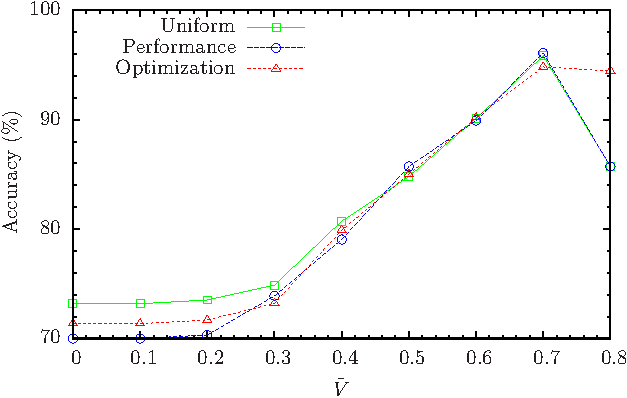
\includegraphics[width=.90\linewidth]{../Figure/threshould_accuracy}
  \caption{Classification Accuracy}
  \label{fig:threshould_accuracy}
\end{subfigure}%
\begin{subfigure}{.40\textwidth}
  \centering
  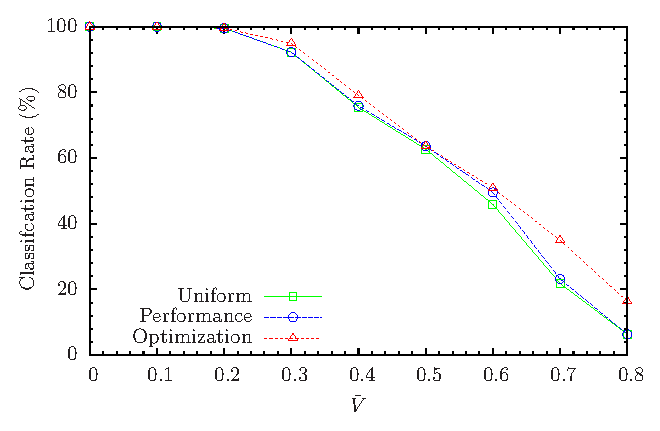
\includegraphics[width=.90\linewidth]{../Figure/threshould_rate}
  \caption{Classification Rate}
  \label{fig:threshould_rate}
\end{subfigure}
\caption{Classification accuracy and rates for different $C\text{-strategy}$ methods in different $\bar{V}$ values.}
\label{fig:threshoulds}
\end{figure}

